\documentclass[JCDReport.tex]{subfiles} 
\begin{document}


% Give a short description (1-2 paragraphs) of what VFS Core is.
The VFSBase is the base of the file system. It implements the functionality to creating, renaming, deleting, importing, exporting, files and folders. It also provides functionality to query disk information like free space or occupied space. To store the files, there are several compression and encryption options available. Additionally, it creates a new version for every action on the file system, and thus provides a history for the file system. The file system also handles big data by storing all the things on the disk instead of storing them in the RAM before writing it to the disk.

\subsection{Requirements}


% Describe which requirements (and possibly bonus requirements) you have implemented in this part. Give a quick description (1-2 sentences) of each requirement. List the software elements (classes and or functions) that are mainly involved in implementing each requirement.

\subsubsection{Introduction: About the FileSystem and the FileSystemTextManipulator}
Most of the features discussed in this section are about the FileSystem and the FileSystemTextManipulator. The first question might be: the FileSystem and the FileSystemTextManipulator are very similar and provide nearly the same interface, why are the separate? The answer to this question is: separation of concerns and encapsulation.\\
The FileSystemTextManipulator provides a \textit{beautiful} interface which is easy to use and to understand. It wraps the FileSystem and abstracts away certain tasks, like converting a given path to an object to the object itself (e.g. it converts "/a/b/c" to the directory object "c"). Also, using the FileSystemTextManipulator, only a certain part of the actual file system is extracted. This way, the file system can handle more files then the RAM size of the current client is. Also, the FileSystemTextManipulator uses some structures only known to the VFSBase assembly, and it encapsulates all the internal objects by only returning values that should be available publicly.\\

The FileSystem is the core of the file system functionality. It implements all the internal structure to store the files and folders to the disk.\\
Finally, there are the ThreadSafeFileSystem and the ThreadSafeFileSystemTextManipulator classes. They also originate from the separation of concerns design principle and provide a thread safe implementation of the FileSystem and the FileSystemTextManipulator respectively. The thread safety is guaranteed through a ReaderWriterLock\footnote{http://msdn.microsoft.com/en-us/library/system.threading.readerwriterlockslim.aspx}, which allows multiple concurrent reads, and exclusive writes.\\

In this section, if the referenced classes are FileSystem and FileSystemTextManipulator, then of course the ThreadSafeFileSystemTextManipulator and the ThreadSafeFileSystem are relevant too. Furthermore, if there is a method FileSystem.\textit{SomeMethod} in the referenced methods, then the Methods ThreadSafeFileSystem.SomeMethod FileSystemTextManipulator.SomeMethod ThreadSafeFileSystemTextManipulator.SomeMethod are not mentioned, but of course, they are relevant too.

% 1. The virtual disk must be stored in a single file in the working directory in the host file system.
\subsubsection{Store data in single file}
All the data is stored in a single file and in blocks. There are logical block numbers, which serve as pointers. All blocks are, once written, immutable to implement the file history.\\
Classes: BlockManipulator, BlockAllocation\\
Methods: BlockManipulator.WriteBlock BlockManipulator.ReadBlock, BlockAllocation.Allocate

% 2. VFS must support the creation of a new disk with the specied maximum size at the specied location in the host le system.
\subsubsection{Creation of new disk}
The file system supports the creation of new disks at a specified location of the host file system. Because the disk size grows dynamically (elastic disk), no maximum size has to be specified\footnote{https://piazza.com/class\#spring2013/252028400l/26}.\\
Classes: FileSystemFactory, FileSystemTextManipulatorFactory\\
Methods: FileSystemTextManipulatorFactory.Create, FileSystemTextManipulatorFactory.Open, FileSystemFactory.Create, FileSystemFactory.Open

% 3. VFS must support several virtual disks in the host le system.
\subsubsection{Several virtual disks in the host file system}
Multiple virtual disks can be created on the host file system.

% 4. VFS must support disposing of the virtual disk.
\subsubsection{Disposing of the virtual disk}
To dispose a virtual disk, the virtual file system can be closed. After closing a file system, the virtual disk can be deleted, as it is a normal file on the host system.\\
Classes: FileSystem, FileSystemTextManipulator\\
Methods: FileSystem.Dispose

% 5. VFS must support creating/deleting/renaming directories and files.
\subsubsection{Creating, deleting, renaming directories and files}
The user can create, delete and rename directories. Files can be imported, and then be renamed or deleted.
Classes: FileSystem, FileSystemTextManipulator\\
Methods:FileSystem.CreateFolder, FileSystem.Rename, FileSystem.Delete

% 6. VFS must support navigation: listing of les and folders, and going to a location expressed by a concrete path.
\subsubsection{Listing and navigation}
The files and folders can be listed and navigated through. The file system supports going to a location expressed by a concrete path.\\
Classes: FileSystem, FileSystemTextManipulator\\
Methods: FileSystem.List, FileSystem.Folders, FileSystem.Files, FileSystem.List

% 7. VFS must support moving/copying directories and les, including hierarchy.
\subsubsection{Moving / copying directories and files}
The files and directories can be copied. Because of the history implementation, some performance optimizations are possible. Thus, the copy time does not depend on the directory or file size, but solely on the directory depth.\\
Classes: FileSystem, FileSystemTextManipulator\\
Methods: FileSystem.Move, FileSystem.Copy

% 8. VFS must support importing files and directories from the host file system.
% 9. VFS must support exporting files and directories to the host le system.
\subsubsection{Import and export}
The VFS supports importing and exporting files and directories from and to the host system respectively. Of course, the import and export functionality is recursive for directories.\\
Classes: FileSystem, FileSystemTextManipulator\\
Methods: FileSystem.Import, FileSystem.Export\\

% 10. VFS must support querying of free/occupied space in the virtual disk.
\subsubsection{Querying of free and occupied space}
The file system allows to query for free and occupied space. The free space corresponds to the free space on the host file system. In the GUI, the view to the free and occupied space can be found in the main menu under "Info"/"Disk Info".\\
Classes: FileSystemOptions\\
Methods: FileSystemOptions.DiskOccupied, FileSystemOptions.DiskFree\\
\begin{figure}[h!]
	\centering
	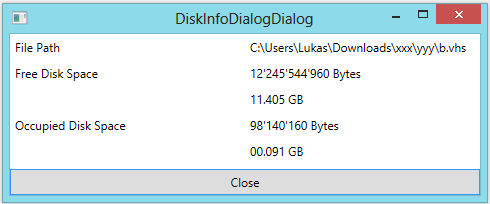
\includegraphics[scale=1]{Images/free_and_occupied_space.png} 
	\caption{Free and occupied space}
\end{figure}

% 1. Compression, if implemented with 3d party library. (1p)
\subsubsection{Compression with 3rd party library}
There are multiple compression types available. One of them is a third party implementation of the Microsoft deflate stream\footnote{http://msdn.microsoft.com/en-us/library/system.io.compression.deflatestream.aspx}.
Patterns: Decorator pattern, Null object pattern (for no encryption)\\
Classes: MicrosoftStreamCompressionStrategy, DeflateStream\\
Methods: DecorateToVFS, DecorateToHost\\
\begin{figure}[h!]
	\centering
	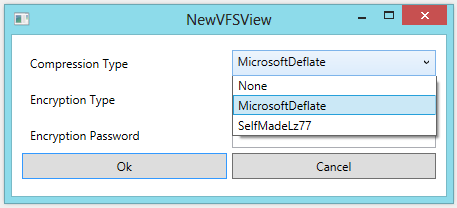
\includegraphics[scale=1]{Images/compression_types.png} 
	\caption{Compression types}
\end{figure}

% 1. Compression, if implemented by hand (you can take a look at the arithmetic compression8). (2p)
\subsubsection{Compression implemented by hand}
Compression by hand is implemented. The basic idea behind the compression is the LZ77 algorithm\footnote{http://www.ieeeghn.org/wiki/index.php/Milestones:Lempel-Ziv\_Data\_Compression\_Algorithm,\_1977}.\\
Patterns: Decorator pattern, Null object pattern (for no encryption)\\
Classes: SelfMadeLz77Stream, Lz77Triple, Lz77Constants, CircularBuffer, SelfMadeLz77StreamCompressionStrategy\\
Methods: SelfMadeLz77Stream.Read, SelfMadeLz77Stream.Write

% 2. Encryption, if implemented with 3d party library. (1p)
\subsubsection{Encryption with 3rd party library}
There are multiple encryption types available. One of them is a third party implementation of the Microsoft Rijndael, the AES standard\footnote{http://msdn.microsoft.com/en-us/library/system.security.cryptography.rijndael.aspx}.\\
Additionally, the encryption needs a user defined password. This password is then used to calculate the encryption / decryption key. This means, that a virtual disk without this password cannot be decrypted.
Patterns: Decorator pattern, Null object pattern (for no encryption)\\
Classes: Rijndael\\
\begin{figure}[h!]
	\centering
	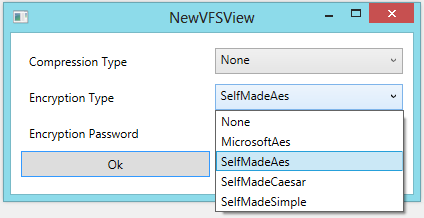
\includegraphics[scale=1]{Images/encryption_types.png} 
	\caption{Encryption types}
\end{figure}

% 2. Encryption, if implemented by hand. (3p)
\subsubsection{Encryption implemented by hand}
Encryption was also implemented by hand. There is a simple encryption and a caesar encryption which are fast, but very weak. Therefore, the AES-256 with CBC\footnote{part of the AES standard, http://csrc.nist.gov/publications/fips/fips197/fips-197.pdf} was implemented.\\
Patterns: Decorator pattern, Null object pattern (for no encryption)\\
Additionally, the encryption needs a user defined password. This password is then used to calculate the encryption / decryption key. This means, that a virtual disk without this password cannot be decrypted.\\
Classes: SelfMadeAes256Cryptor, AesHelperMethods, AesConstants\\
Methods: SelfMadeAes256Cryptor.EncryptBlocks, SelfMadeAes256Cryptor.DecryptBlocks

% 3. Elastic disk: Virtual disk can dynamically grow or shrink, depending on its occupied space. (2p)
\subsubsection{Elastic disk}
The elastic disk is implemented. The file system only allocates disk space when it is required and there are no "practical" limit for the file size or the disk size. It probably will be limited either by the host file system or the hardware itself. The file system is designed in such a way that it does not need to reorganize itself to be fast (known as defragmentation).\\
Classes: BlockAllocation\\
Methods: BlockAllocation.Allocate

% 3. Large data: This means, that VFS core can store & operate amount of data, that can't t to PC RAM ( typically, more than 4Gb). (3p)
\subsubsection{Large data}
As mentioned above, large data is supported. File contents are written directly to the disk, and does not store whole files in memory. Therefore, the file system does not need much RAM, but can handle huge files tough.\\
Classes: BlockManipulator, FileSystem, FileSystemTextManipulator\\
Methods: BlockManipulator.WriteBlock, BlockManipulator.ReadBlock, FileSystem.Import, FileSystem.Export



% 
%\subsubsection{TODO}
%TODO.\\
%Classes:\\
%Methods:\\
%\begin{figure}[h!]
%	\centering
%	
\includegraphics[scale=1]{Images/todo.png} 
%	\caption{TODO}
%\end{figure}




\subsection{Design}

% TODO: Remove this text and replace it with actual content
% Give an overview of the design of this part and describe in general terms how the implementation works. You can mention design patterns used, class diagrams, definition of custom file formats, network protocols, or anything else that helps understand the implementation.

\subsection{File Format}

The design of the file format is related to the Unix File System (UFS)\footnote{http://en.wikipedia.org/wiki/Unix\_File\_System} and the New Technology File System (NTFS)\footnote{http://en.wikipedia.org/wiki/NTFS}. The file is partitioned into two sections:

\begin{itemize}
  \item one super block
  \item many normal blocks
\end{itemize}

\begin{figure}[h!]
  \framebox(100,20){Super block}
  \put(0,0){\framebox(290,20){Normal blocks}}
  \put(0,-20){\framebox(15,20){$b_{1}$}}
  \put(15,-20){\framebox(15,20){$b_{2}$}}
  \put(30,-20){\framebox(15,20){$b_{3}$}}
  \put(45,-20){\framebox(245,20){...}}
  \put(275,-20){\framebox(15,20){$b_{n}$}}
  \caption{Partitions of the virtual disk with $n$ normal blocks.}
\end{figure}


\subsubsection{Super Block}

The super block has a constant size of 32 KB. Although most of the space is not needed yet, it can be used to save meta information about the file system:
\begin{itemize}
  \item block number of the latest root node
  \item used block amount and block size\\
  ($block\_amount * block\_size + super\_block\_size = disk\_size$)
  \item version of the current file (for file history)
  \item version of the file format
  \item ID of the virtual disk (for synchronization)
  \item selected compression algorithm
  \item file encryption algorithm(s)
  \item encrypted key for file encryption
  \item hashed seed/password for file encryption
  \item etc.
\end{itemize}

\subsubsection{Normal Blocks}

The normal blocks consist of many blocks of a fixed block size (e.g. 8KB). The block size is stored in the file system meta information, which is stored in the super block. The block size is the same for every block and cannot be changed after creating the file. Though the block size could be configured at creation time of the disk, which is not available in the GUI, because it was not a requirement.

\paragraph{Normal Block Types} ~\\

\noindent One normal block can be of one of the following types:

\begin{itemize}
  \item Index Node
    \item File Node
    \item Folder Node
  \item Indirect Node
  \item File Content Node
\end{itemize}

\paragraph{Index Node} ~\\

The Index Node contains the file type (file or directory, 1 byte) and the name (max. 255 bytes, can contain any character excluding '/' and '$\backslash0$') of one object. The next 64 bytes contain the block count of the blocks, which are referenced  (through the Indirection Nodes) by this Index node. The next 64 bytes contain the indirection node number, which is a reference to the indirection node. The next 64 bytes are reserved for the version of the object (important for the history implementation). The next 64 bytes are reserved for the predecessor object reference (also for the history implementation).\\
If the Index Node is a file, then the next 32 byte describe the length of the last block, so the file system knows which data of the last block is relevant.\\
If the Index Node is a folder, then the next 64 bytes describe the amount of blocks used. This is important for the root folder and the synchronization.\\

The latest root node can be at any position. The reference to the root node is stored in the options, which are stored in the master block size. The root node is a special folder without a name. The latest root node always has a back reference to the previous root node, unless it is the first root node with version 0.

The block $b_{1}$ is reserved for other meta information, also organized as a folder. Until now, this block is unused, but it might be useful in the future.\\

If the file type is a directory, then the Index Node contains references to an other Index Nodes (files and directories). These are considered sub-files and sub-directories.\\

If the file type is a file, then the Index Node contains references to File Content Nodes. These File Content Nodes must be accessible in the same order they were put into the file system. Because of the concept of the Indirection Nodes, random access is possible. Therefore, seeking to any block in the file takes $\mathcal{O}(1)$, which is very good, especially if only a very small part of a huge file is needed.\\

The File Content Node contains only file content. This content can be encrypted and/or compressed. The last content node of a file is filled with a padding, so block numbers can identify blocks in the file system. If only very small files are stored, it is recommended to reduce the block size.\\

The Indirect Nodes are used to address multiple blocks. There are three levels of Indirect Nodes. First, the one which is referenced by the Index Node (File Node or Folder Node), is the 1st level Indirect Node. This one references to multiple 2nd level indirect nodes. Any of the 2nd level Indirect Nodes references to multiple 3rd Indirect Nodes. And every 3rd Indirect Node references to multiple blocks, which are of type Index Node. For folders, these addressed blocks are File Nodes or Folder Nodes. For files, these addressed blocks are File Content Nodes.


\subsection{Formulas}

\begin{equation}
{block\ reference\ size} = {64\ Byte} = sizeof(long)
\end{equation}

\begin{equation}
references\ per\ Indirect Node = \cfrac{block\ size}{block\ reference\ size}
\end{equation}

\begin{equation}
\begin{split}
maximal\ file\ size =
  \bigg(\cfrac{block\ size}{block\ reference\ size}\bigg)^3\\
\end{split}
\end{equation}

\begin{equation}
maximal\ amount\ of\ blocks = 2^{block\ reference\ size}
\end{equation}


\subsection{Implementation}

Most of the basic file system implementation can be found in the VFSBase project. The VFSBlockAbstraction abstracts all the block operations, so the VFSBase can use the block abstraction and write any data to any block which can be addressed with a block number.\\

Therefore the VFSBase depends on the VFSBlockAbstraction. Additionally, the VFSBase depends on the VFSWCFContracts project, where the interface of the WCF disk service and the Data Transfer Objects (DTOs) are defined.

\begin{figure}[h!]
	\centering
	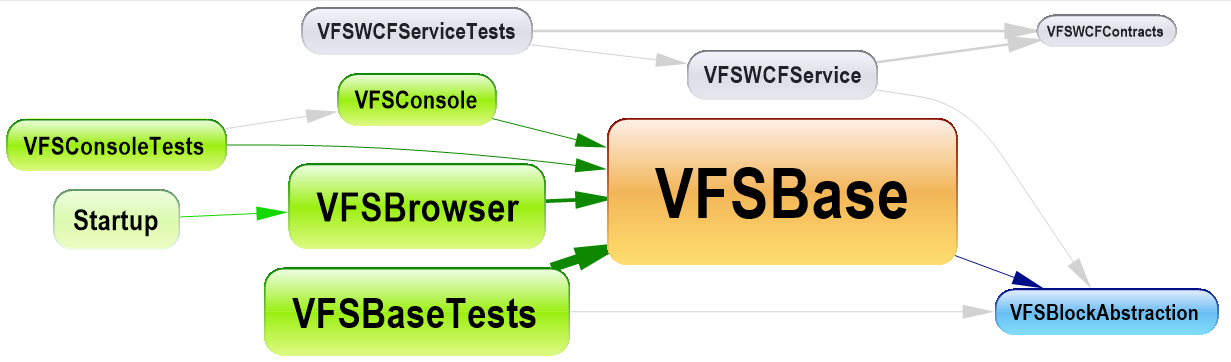
\includegraphics[scale=0.45]{Images/vfsbase_dependency_diagram.png} 
	\caption{Dependencies of the VFSBase}
\end{figure}



\end{document}

